% Options for packages loaded elsewhere
\PassOptionsToPackage{unicode}{hyperref}
\PassOptionsToPackage{hyphens}{url}
\PassOptionsToPackage{dvipsnames,svgnames,x11names}{xcolor}
%
\documentclass[
  letterpaper,
  DIV=11,
  numbers=noendperiod]{scrartcl}

\usepackage{amsmath,amssymb}
\usepackage{iftex}
\ifPDFTeX
  \usepackage[T1]{fontenc}
  \usepackage[utf8]{inputenc}
  \usepackage{textcomp} % provide euro and other symbols
\else % if luatex or xetex
  \usepackage{unicode-math}
  \defaultfontfeatures{Scale=MatchLowercase}
  \defaultfontfeatures[\rmfamily]{Ligatures=TeX,Scale=1}
\fi
\usepackage{lmodern}
\ifPDFTeX\else  
    % xetex/luatex font selection
\fi
% Use upquote if available, for straight quotes in verbatim environments
\IfFileExists{upquote.sty}{\usepackage{upquote}}{}
\IfFileExists{microtype.sty}{% use microtype if available
  \usepackage[]{microtype}
  \UseMicrotypeSet[protrusion]{basicmath} % disable protrusion for tt fonts
}{}
\makeatletter
\@ifundefined{KOMAClassName}{% if non-KOMA class
  \IfFileExists{parskip.sty}{%
    \usepackage{parskip}
  }{% else
    \setlength{\parindent}{0pt}
    \setlength{\parskip}{6pt plus 2pt minus 1pt}}
}{% if KOMA class
  \KOMAoptions{parskip=half}}
\makeatother
\usepackage{xcolor}
\setlength{\emergencystretch}{3em} % prevent overfull lines
\setcounter{secnumdepth}{-\maxdimen} % remove section numbering
% Make \paragraph and \subparagraph free-standing
\makeatletter
\ifx\paragraph\undefined\else
  \let\oldparagraph\paragraph
  \renewcommand{\paragraph}{
    \@ifstar
      \xxxParagraphStar
      \xxxParagraphNoStar
  }
  \newcommand{\xxxParagraphStar}[1]{\oldparagraph*{#1}\mbox{}}
  \newcommand{\xxxParagraphNoStar}[1]{\oldparagraph{#1}\mbox{}}
\fi
\ifx\subparagraph\undefined\else
  \let\oldsubparagraph\subparagraph
  \renewcommand{\subparagraph}{
    \@ifstar
      \xxxSubParagraphStar
      \xxxSubParagraphNoStar
  }
  \newcommand{\xxxSubParagraphStar}[1]{\oldsubparagraph*{#1}\mbox{}}
  \newcommand{\xxxSubParagraphNoStar}[1]{\oldsubparagraph{#1}\mbox{}}
\fi
\makeatother

\usepackage{color}
\usepackage{fancyvrb}
\newcommand{\VerbBar}{|}
\newcommand{\VERB}{\Verb[commandchars=\\\{\}]}
\DefineVerbatimEnvironment{Highlighting}{Verbatim}{commandchars=\\\{\}}
% Add ',fontsize=\small' for more characters per line
\usepackage{framed}
\definecolor{shadecolor}{RGB}{241,243,245}
\newenvironment{Shaded}{\begin{snugshade}}{\end{snugshade}}
\newcommand{\AlertTok}[1]{\textcolor[rgb]{0.68,0.00,0.00}{#1}}
\newcommand{\AnnotationTok}[1]{\textcolor[rgb]{0.37,0.37,0.37}{#1}}
\newcommand{\AttributeTok}[1]{\textcolor[rgb]{0.40,0.45,0.13}{#1}}
\newcommand{\BaseNTok}[1]{\textcolor[rgb]{0.68,0.00,0.00}{#1}}
\newcommand{\BuiltInTok}[1]{\textcolor[rgb]{0.00,0.23,0.31}{#1}}
\newcommand{\CharTok}[1]{\textcolor[rgb]{0.13,0.47,0.30}{#1}}
\newcommand{\CommentTok}[1]{\textcolor[rgb]{0.37,0.37,0.37}{#1}}
\newcommand{\CommentVarTok}[1]{\textcolor[rgb]{0.37,0.37,0.37}{\textit{#1}}}
\newcommand{\ConstantTok}[1]{\textcolor[rgb]{0.56,0.35,0.01}{#1}}
\newcommand{\ControlFlowTok}[1]{\textcolor[rgb]{0.00,0.23,0.31}{\textbf{#1}}}
\newcommand{\DataTypeTok}[1]{\textcolor[rgb]{0.68,0.00,0.00}{#1}}
\newcommand{\DecValTok}[1]{\textcolor[rgb]{0.68,0.00,0.00}{#1}}
\newcommand{\DocumentationTok}[1]{\textcolor[rgb]{0.37,0.37,0.37}{\textit{#1}}}
\newcommand{\ErrorTok}[1]{\textcolor[rgb]{0.68,0.00,0.00}{#1}}
\newcommand{\ExtensionTok}[1]{\textcolor[rgb]{0.00,0.23,0.31}{#1}}
\newcommand{\FloatTok}[1]{\textcolor[rgb]{0.68,0.00,0.00}{#1}}
\newcommand{\FunctionTok}[1]{\textcolor[rgb]{0.28,0.35,0.67}{#1}}
\newcommand{\ImportTok}[1]{\textcolor[rgb]{0.00,0.46,0.62}{#1}}
\newcommand{\InformationTok}[1]{\textcolor[rgb]{0.37,0.37,0.37}{#1}}
\newcommand{\KeywordTok}[1]{\textcolor[rgb]{0.00,0.23,0.31}{\textbf{#1}}}
\newcommand{\NormalTok}[1]{\textcolor[rgb]{0.00,0.23,0.31}{#1}}
\newcommand{\OperatorTok}[1]{\textcolor[rgb]{0.37,0.37,0.37}{#1}}
\newcommand{\OtherTok}[1]{\textcolor[rgb]{0.00,0.23,0.31}{#1}}
\newcommand{\PreprocessorTok}[1]{\textcolor[rgb]{0.68,0.00,0.00}{#1}}
\newcommand{\RegionMarkerTok}[1]{\textcolor[rgb]{0.00,0.23,0.31}{#1}}
\newcommand{\SpecialCharTok}[1]{\textcolor[rgb]{0.37,0.37,0.37}{#1}}
\newcommand{\SpecialStringTok}[1]{\textcolor[rgb]{0.13,0.47,0.30}{#1}}
\newcommand{\StringTok}[1]{\textcolor[rgb]{0.13,0.47,0.30}{#1}}
\newcommand{\VariableTok}[1]{\textcolor[rgb]{0.07,0.07,0.07}{#1}}
\newcommand{\VerbatimStringTok}[1]{\textcolor[rgb]{0.13,0.47,0.30}{#1}}
\newcommand{\WarningTok}[1]{\textcolor[rgb]{0.37,0.37,0.37}{\textit{#1}}}

\providecommand{\tightlist}{%
  \setlength{\itemsep}{0pt}\setlength{\parskip}{0pt}}\usepackage{longtable,booktabs,array}
\usepackage{calc} % for calculating minipage widths
% Correct order of tables after \paragraph or \subparagraph
\usepackage{etoolbox}
\makeatletter
\patchcmd\longtable{\par}{\if@noskipsec\mbox{}\fi\par}{}{}
\makeatother
% Allow footnotes in longtable head/foot
\IfFileExists{footnotehyper.sty}{\usepackage{footnotehyper}}{\usepackage{footnote}}
\makesavenoteenv{longtable}
\usepackage{graphicx}
\makeatletter
\def\maxwidth{\ifdim\Gin@nat@width>\linewidth\linewidth\else\Gin@nat@width\fi}
\def\maxheight{\ifdim\Gin@nat@height>\textheight\textheight\else\Gin@nat@height\fi}
\makeatother
% Scale images if necessary, so that they will not overflow the page
% margins by default, and it is still possible to overwrite the defaults
% using explicit options in \includegraphics[width, height, ...]{}
\setkeys{Gin}{width=\maxwidth,height=\maxheight,keepaspectratio}
% Set default figure placement to htbp
\makeatletter
\def\fps@figure{htbp}
\makeatother
% definitions for citeproc citations
\NewDocumentCommand\citeproctext{}{}
\NewDocumentCommand\citeproc{mm}{%
  \begingroup\def\citeproctext{#2}\cite{#1}\endgroup}
\makeatletter
 % allow citations to break across lines
 \let\@cite@ofmt\@firstofone
 % avoid brackets around text for \cite:
 \def\@biblabel#1{}
 \def\@cite#1#2{{#1\if@tempswa , #2\fi}}
\makeatother
\newlength{\cslhangindent}
\setlength{\cslhangindent}{1.5em}
\newlength{\csllabelwidth}
\setlength{\csllabelwidth}{3em}
\newenvironment{CSLReferences}[2] % #1 hanging-indent, #2 entry-spacing
 {\begin{list}{}{%
  \setlength{\itemindent}{0pt}
  \setlength{\leftmargin}{0pt}
  \setlength{\parsep}{0pt}
  % turn on hanging indent if param 1 is 1
  \ifodd #1
   \setlength{\leftmargin}{\cslhangindent}
   \setlength{\itemindent}{-1\cslhangindent}
  \fi
  % set entry spacing
  \setlength{\itemsep}{#2\baselineskip}}}
 {\end{list}}
\usepackage{calc}
\newcommand{\CSLBlock}[1]{\hfill\break\parbox[t]{\linewidth}{\strut\ignorespaces#1\strut}}
\newcommand{\CSLLeftMargin}[1]{\parbox[t]{\csllabelwidth}{\strut#1\strut}}
\newcommand{\CSLRightInline}[1]{\parbox[t]{\linewidth - \csllabelwidth}{\strut#1\strut}}
\newcommand{\CSLIndent}[1]{\hspace{\cslhangindent}#1}

\KOMAoption{captions}{tableheading}
\makeatletter
\@ifpackageloaded{caption}{}{\usepackage{caption}}
\AtBeginDocument{%
\ifdefined\contentsname
  \renewcommand*\contentsname{Table of contents}
\else
  \newcommand\contentsname{Table of contents}
\fi
\ifdefined\listfigurename
  \renewcommand*\listfigurename{List of Figures}
\else
  \newcommand\listfigurename{List of Figures}
\fi
\ifdefined\listtablename
  \renewcommand*\listtablename{List of Tables}
\else
  \newcommand\listtablename{List of Tables}
\fi
\ifdefined\figurename
  \renewcommand*\figurename{Figure}
\else
  \newcommand\figurename{Figure}
\fi
\ifdefined\tablename
  \renewcommand*\tablename{Table}
\else
  \newcommand\tablename{Table}
\fi
}
\@ifpackageloaded{float}{}{\usepackage{float}}
\floatstyle{ruled}
\@ifundefined{c@chapter}{\newfloat{codelisting}{h}{lop}}{\newfloat{codelisting}{h}{lop}[chapter]}
\floatname{codelisting}{Listing}
\newcommand*\listoflistings{\listof{codelisting}{List of Listings}}
\makeatother
\makeatletter
\makeatother
\makeatletter
\@ifpackageloaded{caption}{}{\usepackage{caption}}
\@ifpackageloaded{subcaption}{}{\usepackage{subcaption}}
\makeatother

\ifLuaTeX
  \usepackage{selnolig}  % disable illegal ligatures
\fi
\usepackage{bookmark}

\IfFileExists{xurl.sty}{\usepackage{xurl}}{} % add URL line breaks if available
\urlstyle{same} % disable monospaced font for URLs
\hypersetup{
  pdftitle={Shifts in Values, Shifts in Democracy},
  pdfauthor={Jason Gordon},
  colorlinks=true,
  linkcolor={blue},
  filecolor={Maroon},
  citecolor={Blue},
  urlcolor={Blue},
  pdfcreator={LaTeX via pandoc}}


\title{Shifts in Values, Shifts in Democracy}
\usepackage{etoolbox}
\makeatletter
\providecommand{\subtitle}[1]{% add subtitle to \maketitle
  \apptocmd{\@title}{\par {\large #1 \par}}{}{}
}
\makeatother
\subtitle{Identifying Correlations between World Values Survey Responses
and Level of Electoral Democracy}
\author{Jason Gordon}
\date{2025-03-13}

\begin{document}
\maketitle


\newpage

\subsection{Intoduction}\label{intoduction}

Democratic backsliding has increasingly taken hold of the world, with
the Varieties of Democracy (V-DEM) 2024 Democracy Report identifying 28
cases of backsliding in democracies, 13 of which having reverted to
autocracies since the episode began.\footnote{Marina Nord et al.,
  {``Democracy {Report} 2024: {Democracy Winning} and {Losing} at the
  {Ballot}''} (University of Gothenburg: V-Dem Institute, March 2024).}
As backsliding occurs within democracies with elected leaders, there is
seemingly popular support \emph{against} democracy in these countries
--- at least given the results of these elections. So, what shifts in an
electorate's values are the most important to backsliding, and can we
use machine learning techniques to predict the onset of backsliding?

In this paper, I plan to inspect if the wave of autocratization in
democracies is the result of a shift in values against democracy, and
which values are the most important for the shift to autocracy. As the
number of cases of backsliding increases, it becomes increasingly
important to understand why people would vote for actors that seek to
challenge the core foundation of democratic institutions; with this
knowledge, we may be able to further understand when cases of
backsliding can happen.

First, I will be summarizing existing literature on democratic
backsliding, identifying the tension in what causes backsliding. Then, I
will conduct some exploratory data analysis and model fitting of my
dataset, using Lasso to identify notable variables. Finally, I will
discuss if these variables have importance in conducting future
research.

\subsection{Existing Literature}\label{existing-literature}

Over the past twenty-five years, there has been considerable discussion
about the causes of democratic backsliding - defined generally as the
gradual breakdown of democratic institutions through nonviolent --- and
often, legal --- means.\footnote{Stephan Haggard and Robert Kaufman,
  \emph{Backsliding: {Democratic Regress} in the {Contemporary World}},
  Elements in {Political Economy} 9 (Cambridge University Press, 2021);
  Steven Levitsky and Daniel Ziblatt, \emph{How {Democracies Die}},
  First edition (New York: Crown, 2018).} Most discussions claim
polarization is the core idea behind why democracies denigrate, but
little is known about the shifts in values to \emph{why} it happens.

Haggard and Kaufman (2021a) discuss backsliding through the lens of
dysfunction of a lack of trust in institutions, which permit autocrats
to capture the executive.\footnote{Stephan Haggard and Robert Kaufman,
  {``The {Anatomy} of {Democratic Backsliding},''} \emph{Journal of
  Democracy} 32, no. 4 (2021): 27--41.} These scholars point to an
overall frustration with the system leading to polarization, as
anti-system actors may be able to succeed in taking power if the
population has no faith that the system will perform well with them.
Other literature seems to correlate parts of this claim, with Cooley and
Nexon (2020) arguing that these are akin to a ``counter-order''
movement, made in rejection to the liberal system of
ordering.\footnote{Alexander Cooley and Daniel Nexon, \emph{Exit from
  {Hegemony}: {The Unraveling} of the {American Global Order}} (Oxford,
  New York: Oxford University Press, 2020).} Generally, these scholars
agree that movements and politicians rejecting the structure of
governance as it stands currently obtain success, with Haggard and
Kaufman finding it is due to dissatisfaction in institutions.

However, Carothers and Press (2022) expand on this discussion, first
limiting their discussion to the Global South and post-communist Europe,
and delivering three separate categories of democratic backsliding, all
of which create differing interpretations of the values behind
backsliding. They state that backsliding can be caused by
grievance-fueled illiberalism, agreeing with future literature that
frustrations in institutions can drive backsliding; opportunistic
authoritarianism, where autocrats act as political entrepreneurs to
obtain power; and entrenched-interest revanchinism, where an interest
group uses undemocratic means to reassert its claim.\footnote{Thomas
  Carothers and Benjamin Press, {``Understanding and {Responding} to
  {Global Democratic Backsliding}''} (Carnegie Endowment for
  International Peace, October 2022).} Carothers and Press's framework
gives an idea for the potential variance in the viewpoints behind
backsliding, claiming it is not as simple as people being mad about
institutions failing them.

An additional perspective claims that backsliding isn't domestic in
nature, but international. One such scholar, Anna Meyerrose (2020;
2021), finds that instead of backsliding being triggered by domestic
parties, that international organizations (IOs) are to blame. She claims
that because IOs focus on elections and an increase in executive power
in their democracy promotion, in addition to removing some areas of
policy for political parties to divide on, potential autocrats have an
easier time gaining and maintaining power.\footnote{Anna M. Meyerrose,
  {``International {Sources} of {Democratic Backsliding},''} in
  \emph{Routledge {Handbook} of {Illiberalism}} (Routledge, 2021); Anna
  M. Meyerrose, {``The {Unintended Consequences} of {Democracy
  Promotion}: {International Organizations} and {Democratic
  Backsliding},''} \emph{Comparative Political Studies} 53, no. 10-11
  (September 2020): 1547--81,
  \url{https://doi.org/10.1177/0010414019897689}.} Deviating from other
arguments, this branch of literature finds that while there may be
domestic issues, structural problems make backsliding \emph{much} more
likely. As a result, backsliding may have nothing to do with values
populations have.

I intend to put these differing claims to the test. While I expect that
grievances with institutions play a not insignificant role in democratic
backsliding, I do expect there to be variance in how much of a role it
plays. Some states may backslide due to structural issues, or for
electing a leader who at first may adhere to democratic norms, but then
turn against the system later in their term.

\subsection{Data}\label{data}

I plan to utilize the World Values Survey's (WVS) seventh wave of data
to account for the values I plan to inspect, pairing the averages of
responses with the correlating electoral democracy scores found in the
Varieties of Democracy's (V-DEM) data set.

While both are relatively large sources of data, combining the two
results in just 62 observations; since WVS uses different questions
between years, I cannot discuss it over time, leading to, unfortunately,
a rather limited amount of data to analyze. Despite this, there are few
other limitations between the two data sets. Both plot their results on
a scale, meaning there are no significant outlying values, and they are
both trusted sources of data used across the literature.

While I will focus on all questions in the WVS data, I plan on focusing
on the electoral democracy and regime scores in the V-DEM data set. The
electoral democracy index seeks to identify the structural components in
a democracy; that is, are elections free and fair, and are the rights
required for democratic rule generally followed? Alongside this, I will
be collecting the overall regime type in the data, which puts all states
on a ten-point scale from most to least democratic.

I will also create two additional variables, which I also aim to test to
understand if a state is undergoing democratic backsliding: the
difference in electoral democracy score, and a Boolean value for if a
state is in a period of backsliding, defined below:

\begin{Shaded}
\begin{Highlighting}[]
\NormalTok{workingvdem }\OtherTok{\textless{}{-}} \FunctionTok{tibble}\NormalTok{(vdem) }\SpecialCharTok{|\textgreater{}}
  \FunctionTok{filter}\NormalTok{(year }\SpecialCharTok{\textgreater{}} \DecValTok{1975}\NormalTok{) }\SpecialCharTok{|\textgreater{}}
  \FunctionTok{group\_by}\NormalTok{(country\_text\_id) }\SpecialCharTok{|\textgreater{}}
  \FunctionTok{arrange}\NormalTok{(year) }\SpecialCharTok{|\textgreater{}}
  \FunctionTok{mutate}\NormalTok{(}\AttributeTok{diff\_polyarchy =}\NormalTok{ v2x\_polyarchy }\SpecialCharTok{{-}} \FunctionTok{lag}\NormalTok{(v2x\_polyarchy)) }\SpecialCharTok{|\textgreater{}}
  \CommentTok{\# Backsliding boolean variable.}
  \CommentTok{\# I\textquotesingle{}m quantitatively defining it as having decreased in electoral}
  \CommentTok{\# democracy score by more than .005 and having decreased by at}
  \CommentTok{\# least 0.03 in the last two years.}
  \CommentTok{\# I also filtered so that the regime has to be at least some semblance}
  \CommentTok{\# of an electoral autocracy (at least) so that hard autocracies getting}
  \CommentTok{\# more autocratic aren\textquotesingle{}t included.}
  \FunctionTok{mutate}\NormalTok{(}\AttributeTok{backslided =}\NormalTok{ (diff\_polyarchy }\SpecialCharTok{\textless{}} \SpecialCharTok{{-}}\FloatTok{0.005}\NormalTok{) }\SpecialCharTok{\&}
\NormalTok{           (v2x\_regime\_amb }\SpecialCharTok{\textgreater{}} \DecValTok{2}\NormalTok{) }\SpecialCharTok{\&}
\NormalTok{           (}\FunctionTok{lag}\NormalTok{(v2x\_polyarchy, }\DecValTok{2}\NormalTok{) }\SpecialCharTok{{-}}\NormalTok{ v2x\_polyarchy }\SpecialCharTok{\textgreater{}} \FloatTok{0.03}\NormalTok{)) }\SpecialCharTok{|\textgreater{}}
  \CommentTok{\# Filling it out}
  \FunctionTok{mutate}\NormalTok{(}\AttributeTok{backslided =}\NormalTok{ (diff\_polyarchy }\SpecialCharTok{\textless{}} \SpecialCharTok{{-}}\FloatTok{0.001}\NormalTok{) }\SpecialCharTok{\&}
\NormalTok{           (backslided }\SpecialCharTok{|}
\NormalTok{              ((}\FunctionTok{lag}\NormalTok{(backslided) }\SpecialCharTok{\&} \FunctionTok{lag}\NormalTok{(backslided, }\DecValTok{2}\NormalTok{))}\SpecialCharTok{|}
                 \FunctionTok{lead}\NormalTok{(backslided) }\SpecialCharTok{\&} \FunctionTok{lag}\NormalTok{(backslided) }\SpecialCharTok{|}
                 \FunctionTok{lead}\NormalTok{(backslided, }\DecValTok{2}\NormalTok{) }\SpecialCharTok{\&} \FunctionTok{lead}\NormalTok{(backslided)))) }\SpecialCharTok{|\textgreater{}}
  \FunctionTok{ungroup}\NormalTok{() }\SpecialCharTok{|\textgreater{}}
  \FunctionTok{filter}\NormalTok{(year }\SpecialCharTok{\textgreater{}} \DecValTok{2009}\NormalTok{) }\SpecialCharTok{|\textgreater{}}
  \FunctionTok{arrange}\NormalTok{(country\_text\_id) }\SpecialCharTok{|\textgreater{}}
  \FunctionTok{select}\NormalTok{(country\_name,}
\NormalTok{         country\_text\_id,}
\NormalTok{         year,}
\NormalTok{         v2x\_polyarchy,}
\NormalTok{         v2x\_libdem, }
\NormalTok{         v2x\_regime\_amb, }
\NormalTok{         diff\_polyarchy, }
\NormalTok{         backslided)}
\end{Highlighting}
\end{Shaded}

By defining a period of backsliding in an overall shift from democracy
that does \emph{not} have to be a sharp decline every year, I can create
clear periods of backsliding, easily identifying cases.

In addition to creating these variables, I will be cleaning both data
sets and attempting to standardize missing values if I cannot remove
them, which will hopefully make my data as accurate as possible. This
should also allow me to merge the V-DEM and WVS data without hassle.

\subsubsection{Exploratory Analysis}\label{exploratory-analysis}

To determine which features are the most important to a shift in
electoral democracy score, I plan on using a Lasso model, testing the
electoral democracy score to get the most important variables. While
using the difference in this score may seem more intuitive, its low
variance results in the model being unable to get the top features.

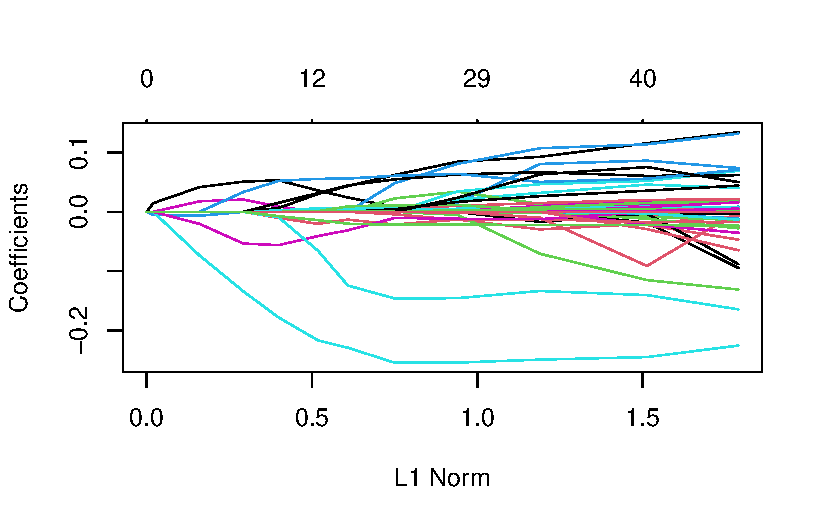
\includegraphics{Episode_2_files/figure-pdf/lassosetup-1.pdf}

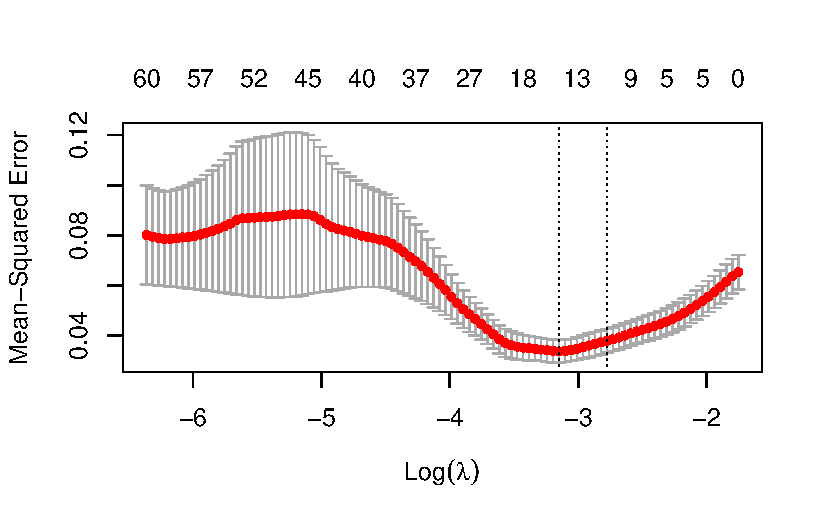
\includegraphics{Episode_2_files/figure-pdf/lassosetup-2.pdf}

Given our cross-validation graph indicates our most important features
will be somewhere between 10 and 15, we can then discuss which variables
are the most important, as seen below.

\begin{Shaded}
\begin{Highlighting}[]
\NormalTok{top\_features }\OtherTok{\textless{}{-}} \FunctionTok{coef}\NormalTok{(cv\_out, }\AttributeTok{s =} \StringTok{"lambda.1se"}\NormalTok{)}
\NormalTok{top\_features }\OtherTok{\textless{}{-}}\NormalTok{ top\_features[}\SpecialCharTok{{-}}\DecValTok{1}\NormalTok{,]}
\NormalTok{top\_features }\OtherTok{\textless{}{-}}\NormalTok{ top\_features[top\_features }\SpecialCharTok{!=} \DecValTok{0}\NormalTok{]}
\FunctionTok{sort}\NormalTok{(}\FunctionTok{abs}\NormalTok{(top\_features), }\AttributeTok{decreasing =} \ConstantTok{TRUE}\NormalTok{) }\SpecialCharTok{|\textgreater{}} \FunctionTok{head}\NormalTok{(}\DecValTok{15}\NormalTok{)}
\end{Highlighting}
\end{Shaded}

\begin{verbatim}
        Q211         Q239          Q38         Q212         Q271         Q225 
0.1967821941 0.0559778577 0.0482793422 0.0480802239 0.0364528223 0.0228602491 
         Q73           Q3        Q292I         Q182         Q262 
0.0190355263 0.0151253037 0.0107729186 0.0044779803 0.0001399158 
\end{verbatim}

Thus, the most impactful questions on the democracy score are as
follows, alongside the graph of how important they are (with further
away from 0 indicating increased important as more factors are added):
\textbf{Q211} \emph{(Openness to attending a political demonstration)}
\textbf{Q239} \emph{(Opinion on religious law governing a country)}
\textbf{Q38} \emph{(Is it a child's duty to take care of a sick
parent?)} \textbf{Q212} \emph{(Openness to joining unofficial strikes)}
\textbf{Q271} \emph{(If the respondent is living with their parents)}
\textbf{Q225} \emph{(Frequency of opposition candidates prevented from
running)} \textbf{Q73} \emph{(Confidence in country's parliament)}
\textbf{Q3} \emph{(Importance of leisure time)} \textbf{Q292I}
\emph{(Belief politicians are incompetent or ineffective)} \textbf{Q182}
\emph{(Is homosexuality justifiable?)} \textbf{Q262} \emph{(Age)}

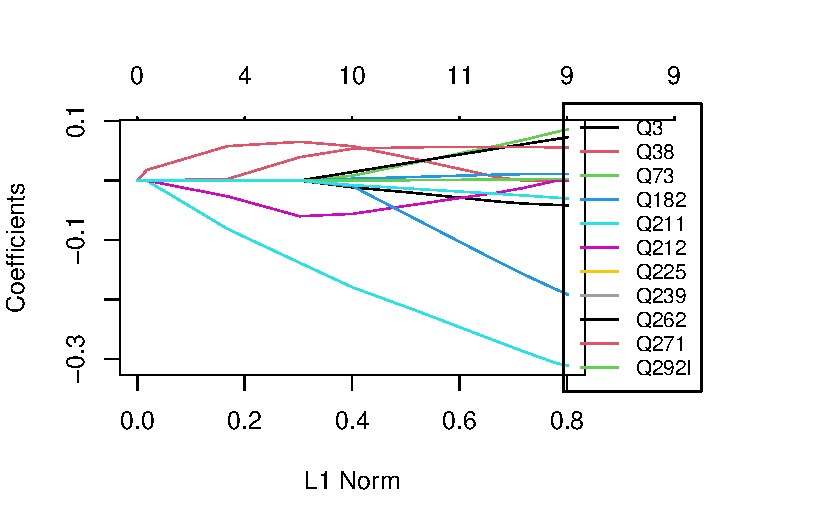
\includegraphics{Episode_2_files/figure-pdf/lassoresults-1.pdf}

Many of these reflect core foundations of democracy, but there are some
that seem more cultural. We can see notable trends in political
demonstrations highly correlating with overall level of electoral
democracy; Q211 and Q212 are among the first variables given
coefficients, and Q211 has the largest overall effect. This makes sense,
as generally, an increased level to take public action for political
reasons would increase the level of accountability leaders have to their
people.

Additionally, Wave 7 denotes variables like confidence in parliament,
belief politicians are incompetent or ineffective, and frequency of
opposition candidates being prevented from running. These all directly
tie into whether electoral democracy is healthy, as if opposition
candidates are not allowed to run, overall level of democracy decreases,
and the last of these variables is one of the metrics V-DEM also
measures to indicate level of electoral democracy.

Finally, the belief that the government and its actors may be
ineffective make sense to discuss both electoral democracy and
backsliding. As a population's trust of its government falls, it often
polarizes and seeks anti-system candidates, resulting in an increased
likelihood of a potential autocrat's election.

\subsection{Modeling}\label{modeling}

To test if I can predict electoral democracy levels and backsliding, I
decided to use decision trees, in an attempt to classify based on the
different variables we got from Lasso. I tested two trees, finding that
there is no major difference between RandomForest and XGBoost for trees,
as seen below:

\begin{Shaded}
\begin{Highlighting}[]
\NormalTok{wf\_set }\OtherTok{\textless{}{-}} \FunctionTok{workflow\_set}\NormalTok{(}
  \AttributeTok{preproc =} \FunctionTok{list}\NormalTok{(rec),}
  \AttributeTok{models =} \FunctionTok{list}\NormalTok{(}
    \AttributeTok{xgboost =}\NormalTok{ model\_xgboost,}
    \AttributeTok{random\_forest =}\NormalTok{ model\_rf100)}
\NormalTok{)}
  
\NormalTok{wf\_set\_fitted }\OtherTok{\textless{}{-}} \FunctionTok{workflow\_map}\NormalTok{(wf\_set, }\StringTok{"fit\_resamples"}\NormalTok{, }\AttributeTok{resamples =}\NormalTok{ cv\_folds)}
\NormalTok{wf\_set\_fitted }\SpecialCharTok{|\textgreater{}} \FunctionTok{collect\_metrics}\NormalTok{()}
\end{Highlighting}
\end{Shaded}

\begin{verbatim}
# A tibble: 4 x 9
  wflow_id          .config preproc model .metric .estimator  mean     n std_err
  <chr>             <chr>   <chr>   <chr> <chr>   <chr>      <dbl> <int>   <dbl>
1 recipe_xgboost    Prepro~ recipe  boos~ rmse    standard   0.160     5  0.0266
2 recipe_xgboost    Prepro~ recipe  boos~ rsq     standard   0.583     5  0.122 
3 recipe_random_fo~ Prepro~ recipe  rand~ rmse    standard   0.172     5  0.0211
4 recipe_random_fo~ Prepro~ recipe  rand~ rsq     standard   0.606     5  0.0954
\end{verbatim}

However, I will use XGBoosted trees to focus on the variables, creating
500 trees in an attempt for increased accuracy. I also plan on tuning
for the learning rate hyperparameter. Below are the results for my
initial model. I will then get the best fit and use it to make our final
predictions, seen compared to our predictions in the graph below. The
red like is a perfect prediction, that is, the prediction is the same as
the actual value.

\begin{Shaded}
\begin{Highlighting}[]
\NormalTok{xg\_grid }\OtherTok{\textless{}{-}} \FunctionTok{grid\_regular}\NormalTok{(}\FunctionTok{learn\_rate}\NormalTok{(), }\AttributeTok{levels =} \DecValTok{5}\NormalTok{)}

\NormalTok{model\_xgboost\_tune }\OtherTok{\textless{}{-}} \FunctionTok{boost\_tree}\NormalTok{(}\AttributeTok{trees =} \DecValTok{500}\NormalTok{, }\AttributeTok{mtry=}\DecValTok{5}\NormalTok{, }\AttributeTok{learn\_rate =} \FunctionTok{tune}\NormalTok{()) }\SpecialCharTok{|\textgreater{}} 
  \FunctionTok{set\_mode}\NormalTok{(}\StringTok{"regression"}\NormalTok{) }\SpecialCharTok{|\textgreater{}} 
  \FunctionTok{set\_engine}\NormalTok{(}\StringTok{"xgboost"}\NormalTok{)}

\NormalTok{wf }\OtherTok{\textless{}{-}} \FunctionTok{workflow}\NormalTok{() }\SpecialCharTok{|\textgreater{}}
  \FunctionTok{add\_model}\NormalTok{(model\_xgboost\_tune) }\SpecialCharTok{|\textgreater{}}
  \FunctionTok{add\_recipe}\NormalTok{(rec)}

\NormalTok{model\_res }\OtherTok{\textless{}{-}}\NormalTok{ wf }\SpecialCharTok{|\textgreater{}}
  \FunctionTok{tune\_grid}\NormalTok{(}\AttributeTok{resamples =}\NormalTok{ cv\_folds,}
            \AttributeTok{grid =}\NormalTok{ xg\_grid,}
            \AttributeTok{control =} \FunctionTok{control\_grid}\NormalTok{(}\AttributeTok{save\_pred =} \ConstantTok{TRUE}\NormalTok{))}
\end{Highlighting}
\end{Shaded}

\begin{verbatim}
> A | warning: A correlation computation is required, but `estimate` is constant and has 0
               standard deviation, resulting in a divide by 0 error. `NA` will be returned.
\end{verbatim}

\begin{verbatim}
There were issues with some computations   A: x1
\end{verbatim}

\begin{verbatim}
There were issues with some computations   A: x5
There were issues with some computations   A: x5
\end{verbatim}

\begin{verbatim}
\end{verbatim}

\begin{Shaded}
\begin{Highlighting}[]
\FunctionTok{collect\_metrics}\NormalTok{(model\_res)}
\end{Highlighting}
\end{Shaded}

\begin{verbatim}
# A tibble: 10 x 7
     learn_rate .metric .estimator    mean     n std_err .config             
          <dbl> <chr>   <chr>        <dbl> <int>   <dbl> <chr>               
 1 0.0000000001 rmse    standard     0.254     5  0.0111 Preprocessor1_Model1
 2 0.0000000001 rsq     standard   NaN         0 NA      Preprocessor1_Model1
 3 0.0000000178 rmse    standard     0.254     5  0.0111 Preprocessor1_Model2
 4 0.0000000178 rsq     standard   NaN         0 NA      Preprocessor1_Model2
 5 0.00000316   rmse    standard     0.254     5  0.0111 Preprocessor1_Model3
 6 0.00000316   rsq     standard     0.582     5  0.109  Preprocessor1_Model3
 7 0.000562     rmse    standard     0.227     5  0.0126 Preprocessor1_Model4
 8 0.000562     rsq     standard     0.574     5  0.106  Preprocessor1_Model4
 9 0.1          rmse    standard     0.184     5  0.0261 Preprocessor1_Model5
10 0.1          rsq     standard     0.500     5  0.0909 Preprocessor1_Model5
\end{verbatim}

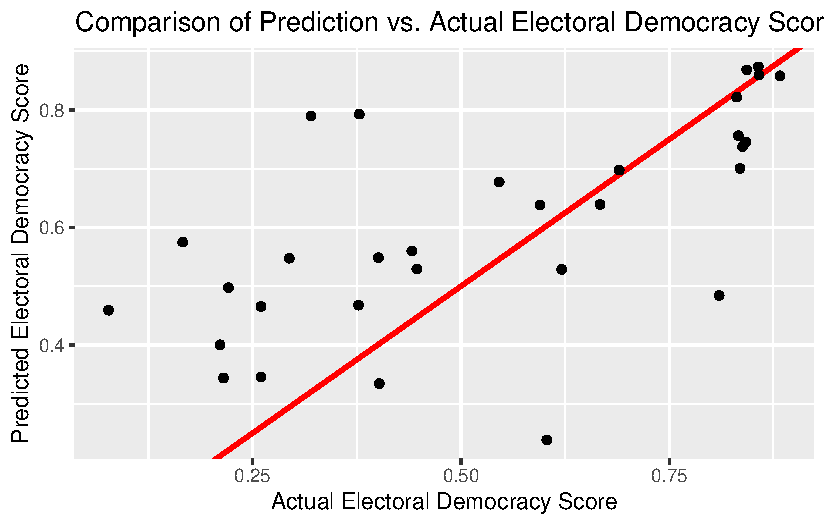
\includegraphics{Episode_2_files/figure-pdf/finalfit-1.pdf}

Seemingly, there is still a large amount of variation in our model,
likely due to a low sample size. A larger sample could predict better -
as the higher electoral democracy scores are a bit more precise - though
there is no way to get this data, as the questions on the World Values
Survey are inconsistent.

I will also attempt to run the model on the full data, in case we missed
any parameters. However, as seen below, there is no significant
difference outside of random shifts due to splitting the entire data.

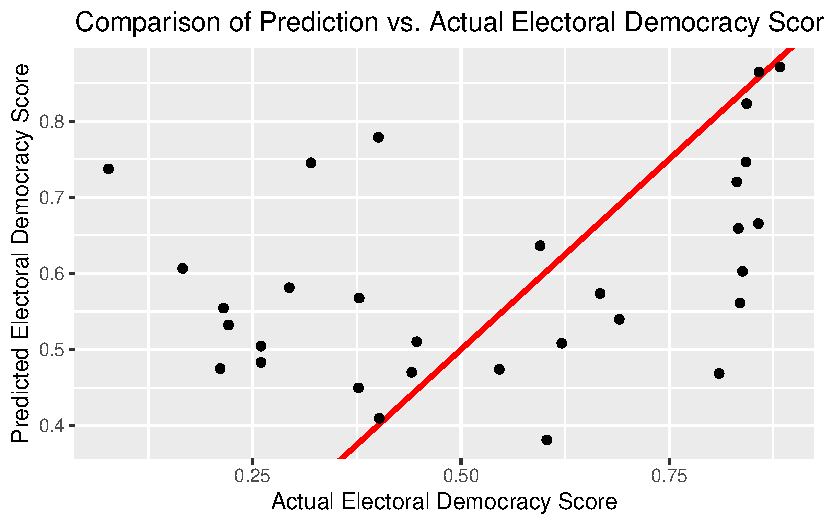
\includegraphics{Episode_2_files/figure-pdf/fulldata-1.pdf}

I also will be testing this model on two more variables: the difference
in electoral democracy score, which indicates backsliding, and the
Boolean variable indicating if a state is in a backsliding episode.
Below is the prediction for difference in electoral democracy score.

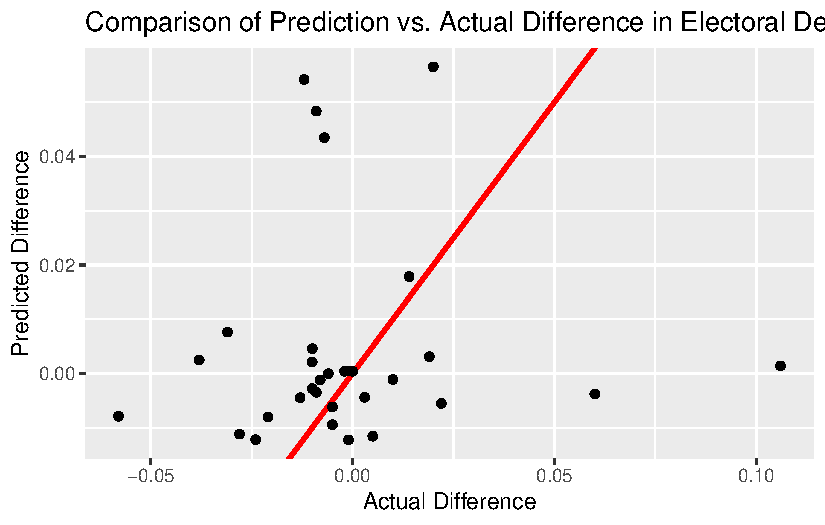
\includegraphics{Episode_2_files/figure-pdf/diffpolyarchy-1.pdf}

Seemingly, the model did decently for differences in electoral democracy
score, but that may be because the actual differences are close to zero,
making it easy for the model to predict. Additionally, we can see if the
model predicts if a state is in an episode of backsliding, with the ROC
Curve below

\begin{verbatim}
> A | warning: No control observations were detected in `truth` with control level 'TRUE'.
\end{verbatim}

\begin{verbatim}
There were issues with some computations   A: x1
There were issues with some computations   A: x1
\end{verbatim}

\begin{verbatim}
\end{verbatim}

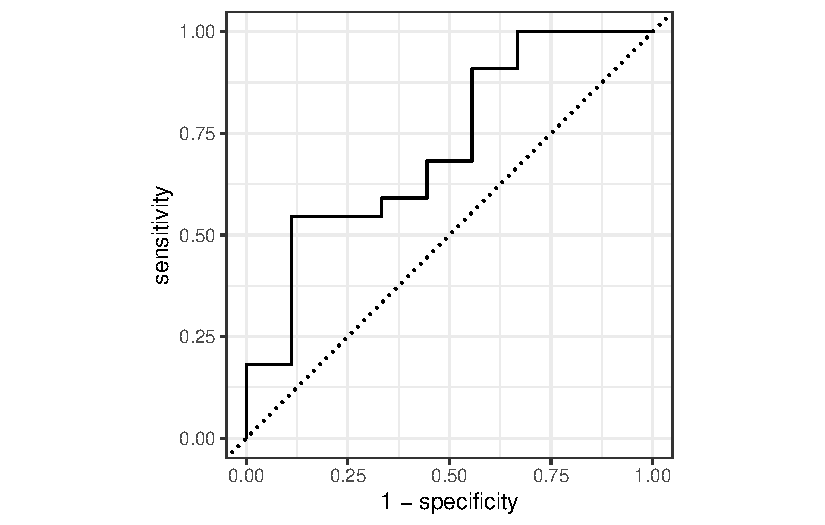
\includegraphics{Episode_2_files/figure-pdf/backslided-1.pdf}

\begin{Shaded}
\begin{Highlighting}[]
\NormalTok{final\_class }\SpecialCharTok{|\textgreater{}} \FunctionTok{collect\_metrics}\NormalTok{()}
\end{Highlighting}
\end{Shaded}

\begin{verbatim}
# A tibble: 3 x 4
  .metric     .estimator .estimate .config             
  <chr>       <chr>          <dbl> <chr>               
1 accuracy    binary         0.645 Preprocessor1_Model1
2 roc_auc     binary         0.283 Preprocessor1_Model1
3 brier_class binary         0.297 Preprocessor1_Model1
\end{verbatim}

Arguably, this data is little better than random selection, with large
steps indicating a small sample size and not much else. With a 64.5\%
accuracy, it may be marginally better than pure random selection, but
likely not by a significant amount.

\subsection{Discussion}\label{discussion}

While the global shift to autocracy is bolstered by an overall
frustration in democratic institutions, it is by no means the only
factor. This research confirms the theoretical claim that backsliding is
correlated with an increase in frustrations with democratic
institutions, but offers other potential variables like democratic
activism and is not a useful predictive model.

Below are the various VIP plots for each model. Here, we can see the
various questions among each graph which may be the most important.

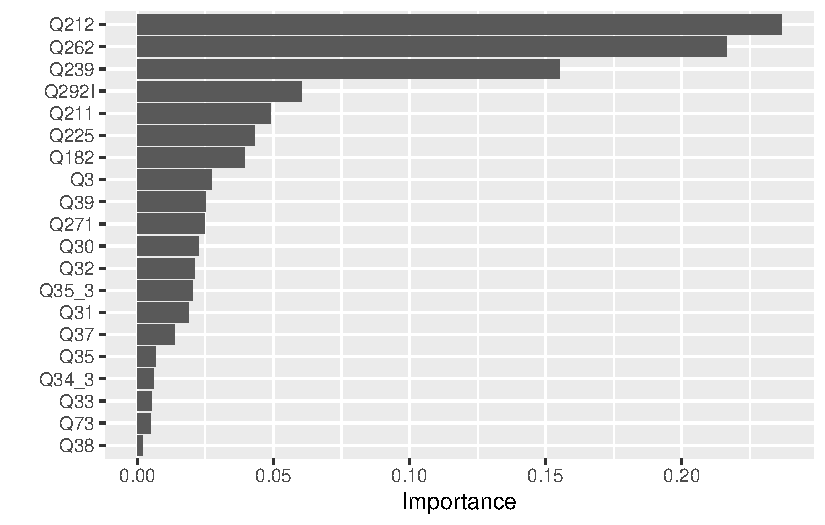
\includegraphics{Episode_2_files/figure-pdf/vip-1.pdf}

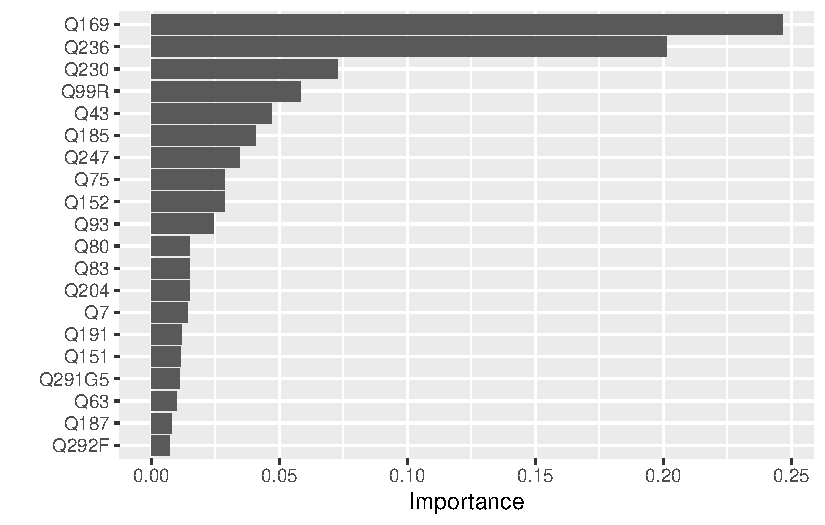
\includegraphics{Episode_2_files/figure-pdf/vip-2.pdf}

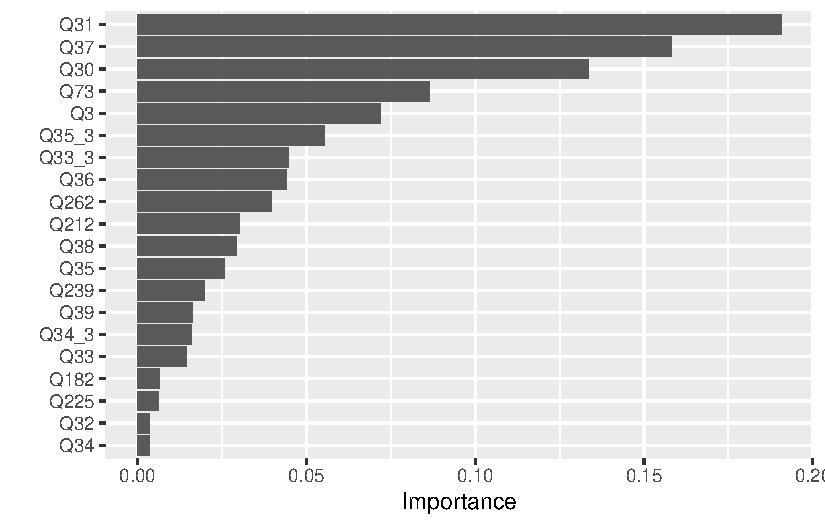
\includegraphics{Episode_2_files/figure-pdf/vip-3.pdf}

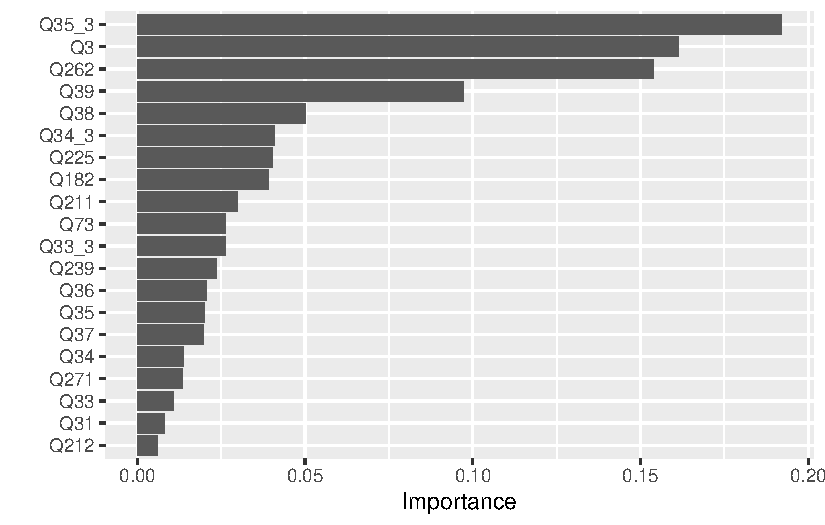
\includegraphics{Episode_2_files/figure-pdf/vip-4.pdf}

The most important features for each model (above 0.1 importance) are as
follows: \textbf{Electoral Democracy Score:} Q212 (Political Action:
Joining Unofficial Strikes), Q211 (Political Action: attending
lawful/peaceful demonstrations), Q239 (Opinion on religious law), Q262
(Age) \textbf{Electoral Democracy Score (with all parameters):} Q291UN3
(The UN usually acts in its own interests), Q209 (Political Action:
signing a petition), Q219 (Political Action Online: encouraging others
to take action) \textbf{Difference in ED Score:} Q33\_3 (Jobs Scarce:
Men should have more right to a job than woken), Q73 (Confidence in
Parliament), Q3 (Important in Life: leisure time), Q31 (Men make better
business executives than women), Q35\_3 (Problem if men have more income
than women) \textbf{Whether a state is in a backsliding episode:} Q35\_3
(Problem if men have more income than women), Q3 (Important in Life:
leisure time), Q39 (People who don't work turn lazy), Q262 (Age)

My initial hypothesis of frustration in institutions causing backsliding
seems to somewhat be important, as confidence in a state's parliament is
important in the model predicting difference in electoral democracy
score, and is flagged in the Lasso prediction, but otherwise, it is
refuted. Instead, gender issues frequent those that are important in
differences in electoral democracy score and backsliding episodes.
However, gendered questions making backsliding more or less likely does
make make sense, as increasing gender gaps drove Donald Trump - someone
who, under his first term, ushered in a period of backsliding - to
victory in November 2024.\footnote{Shane Goldmacher and Lisa Lerer,
  {``Donald {Trump Returns} to {Power}, {Ushering} in {New Era} of
  {Uncertainty},''} \emph{The New York Times}, November 2024; Levitsky
  and Ziblatt, \emph{How {Democracies Die}}.}

However, these results present an additional correlation: that of
democratic activism. In both electoral democracy models, political
activism proved somewhat important multiple times. This correlation
somewhat tracks with the fact that free speech has more restrictions in
more autocratic regimes, but the questions ask if someone is
\emph{willing} to join in the political action, so those states with
higher proportions of people willing to resist likely are more
democratic as a result.

\subsection{Conclusion}\label{conclusion}

Thus, the level of democracy in a state - at least to some extent - is
affected by the values of its population. If people are dissatisfied
with the government and will rarely take political action, an autocratic
regime is more likely, and an increased paternal bias inside a state
correlates with backsliding episodes. Using these correlations, we may
be able to predict backsliding for future states, furthering our
understanding of this shift from democracy in an ever-changing world.

With more resources and time, I may have been able to improve the model
with an increase in data by asking questions like those on the World
Values Survey and gathering an eighth wave of data, effectively doubling
my data set. My challenge - and the one that impacted my results the
most - was a lack of data, since the WVS is taken once every few years
in a single country, and has different questions in each wave. Due to
this, I could only effectively use one wave of data for modeling,
creating difficulties in my model's overall viability. If I could gather
a new set of responses to these questions, I would be able to use that
data to increase my model's accuracy, potentially giving different
results and predicting backsliding episodes more effectively.

\subsection{References}\label{references}

\phantomsection\label{refs}
\begin{CSLReferences}{1}{0}
\bibitem[\citeproctext]{ref-carothersUnderstandingRespondingGlobal2022}
Carothers, Thomas, and Benjamin Press. {``Understanding and {Responding}
to {Global Democratic Backsliding}.''} Carnegie Endowment for
International Peace, October 2022.

\bibitem[\citeproctext]{ref-cooleyExitHegemonyUnraveling2020}
Cooley, Alexander, and Daniel Nexon. \emph{Exit from {Hegemony}: {The
Unraveling} of the {American Global Order}}. Oxford, New York: Oxford
University Press, 2020.

\bibitem[\citeproctext]{ref-goldmacherDonaldTrumpReturns2024}
Goldmacher, Shane, and Lisa Lerer. {``Donald {Trump Returns} to {Power},
{Ushering} in {New Era} of {Uncertainty}.''} \emph{The New York Times},
November 2024.

\bibitem[\citeproctext]{ref-haggardBackslidingDemocraticRegress2021}
Haggard, Stephan, and Robert Kaufman. \emph{Backsliding: {Democratic
Regress} in the {Contemporary World}}. Elements in {Political Economy}
9. Cambridge University Press, 2021.

\bibitem[\citeproctext]{ref-haggardAnatomyDemocraticBacksliding2021}
---------. {``The {Anatomy} of {Democratic Backsliding}.''}
\emph{Journal of Democracy} 32, no. 4 (2021): 27--41.

\bibitem[\citeproctext]{ref-levitskyHowDemocracies2018a}
Levitsky, Steven, and Daniel Ziblatt. \emph{How {Democracies Die}}.
First edition. New York: Crown, 2018.

\bibitem[\citeproctext]{ref-meyerroseInternationalSourcesDemocratic2021}
Meyerrose, Anna M. {``International {Sources} of {Democratic
Backsliding}.''} In \emph{Routledge {Handbook} of {Illiberalism}}.
Routledge, 2021.

\bibitem[\citeproctext]{ref-meyerroseUnintendedConsequencesDemocracy2020}
---------. {``The {Unintended Consequences} of {Democracy Promotion}:
{International Organizations} and {Democratic Backsliding}.''}
\emph{Comparative Political Studies} 53, no. 10-11 (September 2020):
1547--81. \url{https://doi.org/10.1177/0010414019897689}.

\bibitem[\citeproctext]{ref-nordDemocracyReport20242024}
Nord, Marina, Martin Lundstedt, David Altman, Fabio Angiolillo, Cecilia
Borella, Tiago Fernandes, Lisa Gastaldi, Ana Good God, Natalia Natsika,
and Staffan Lindberg. {``Democracy {Report} 2024: {Democracy Winning}
and {Losing} at the {Ballot}.''} University of Gothenburg: V-Dem
Institute, March 2024.

\end{CSLReferences}




\end{document}
